图形学经常与视觉搞混,两者都是利用计算机算法对物理世界的建模。

但图形学(渲染)建模的是图片形成之前的阶段,主要是光线与物体表面交互,光在空气中传输,光最终映射到人眼形成图像。此外图形学还有很多和图像无关的部分,比如角色/物理动画,几何处理等。

而计算机视觉(图像理解,重建)建模的是图像形成之后人脑如何对图像进行理解的过程,从图像中提取特征,识别特定的对象和理解抽象的概念等等。同时,计算机视觉还涉及很多单纯图像的变换,比如图形的滤波,降噪,超分辨率,形变等。

换言之,计算机图形学的兴趣在于物理世界,而计算机视觉的兴趣在于人的视觉理解系统,两者虽然互有涉猎,且在色彩模型和相机模型上有共通知识,但归根到底是不同的学科范畴。

\begin{figure}[H]
    \centering
    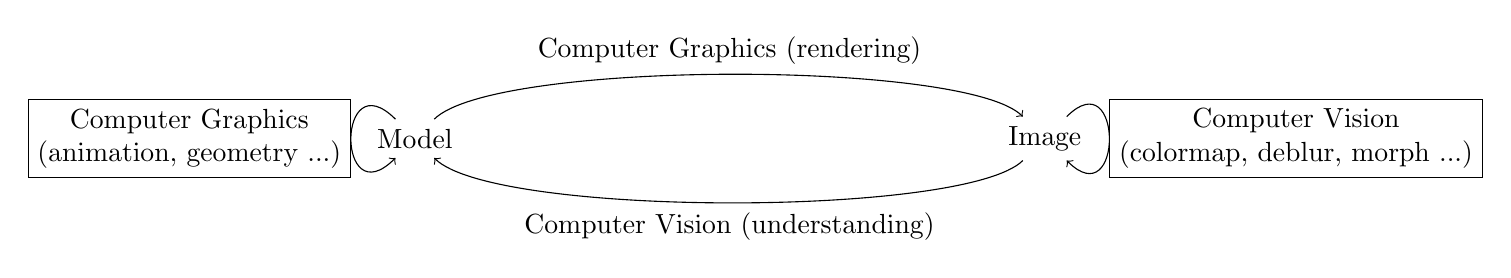
\begin{tikzpicture}[->]
    \node (A) at (0, 0) {Model};
    \node (B) at (8, 0) {Image};
    \draw[->] (A) .. controls (1, 1)
    and (7, 1) .. node[above]{Computer Graphics (rendering)} (B);
    \draw[->] (B) .. controls (7, -1)
    and (1, -1) ..  node[below]{Computer Vision (understanding)} (A);
    \draw[->] (A) .. controls (-1, 1)
    and (-1, -1) ..  node[draw, left, align=center]{Computer Graphics \\ 
    (animation, geometry ...)} (A);
    \draw[->] (B) .. controls (9, 1)
    and (9, -1) ..  node[draw, right, align=center]{Computer Vision \\ 
    (colormap, deblur, morph ...)} (B);
\end{tikzpicture}
    \caption{Difference of CG and CV}
    \label{fig:diff_cg_cv}
\end{figure}